%%%%%%%%%%%%%%%%%%%%%%%
% Cosmological observables
%%%%%%%%%%%%%%%%%%%%%%%
\section{Cosmological observables}
Here we present a brief description of cosmological probes which can be used for constraining dark energy. For more details see e.g. \textcite{weinberg_observational_2013} or \textcite{DE_probes2}.
%In shear-shear tomography, the shear of background galaxies, binned in redshift, is cross correlated. 
%\ssec{Introduction}
%http://terapix.phys.cmu.edu/misc/desc\_feb\_2015\_de\_school\_ShirleyHo.pdf \\
%https://sites.google.com/site/cmucosmos13/lecture-notes \\
%http://arxiv.org/pdf/1201.2434v2.pdf \\

%%%%%%%%%%%%%%%%%%%%%%%
% Cosmic distances
%%%%%%%%%%%%%%%%%%%%%%%
\subsection{Cosmic distances}
In~the~expanding Universe, there are many ways to~specify the~distance between two points due to~the~constantly changing distances and~the~fact that observers look back in~time as they look out in~distance.
\subsubsection{Comoving distance}
The~light traveling along the~$\chi$ direction satisfies the~geodesic equation $\dd s^2=-\dd t^2+a^2(t)\dd \chi^2=0$. The~light emitted at~the~time $t=t_1$ with~$\chi=\chi_1$ (redshift $z$) reaches an~observer at~time $t=t_0$ with~$\chi=0$ (redshift $z=0$). Integrating the~geodesic equation
\eq{
    \label{eq:d_c}
    d_c\equiv\chi_1=\int_0^{\chi_1}\dd\chi=-\int_{t_0}^{t_1}\frac{\dd t}{a(t)}=\frac{1}{H_0}\int_0^z\frac{\dd\tilde z}{E(\tilde z)}\,,
}
where
\eq{
    E(z)\equiv H(z)/H_0=\sqrt{\Omega_{\gamma,0}(z+1)^4+\Omega_{m,0}(z+1)^3+\Omega_{K,0}(z+1)^2+\Omega_{\Lambda,0}}\,.
}
If we expand $E(z)$ around $z=0$ we can write the~cosmic distance as
\eq{
    d_c=\frac{1}{H_0}z-\frac{E'(0)}{2H_0}z^2+\frac{2E'(0)^2-E''(0)}{6H_0}z^3+\mathcal{O}(z^4)\,,
}
where a~prime now (and~for~the~rest of~the~work) represents a~derivative with~respect to~$z$.
\subsubsection{Luminosity distance}
The~luminosity distance $d_L$ is used in~supernovae observations to~link the~supernova luminosity with~the~expansion rate of~the~Universe. It is defined by \parencite{weinberg_observational_2013}
\eq{
    d_L^2\equiv\frac{L_s}{4\pi F}\,,
}
where $L_s$ is the~absolute bolometric (i.e., integrated over all frequencies) luminosity of~a~source, and~$F$ is the~observed bolometric flux. The~flux is defined by $F=L_0/S$, where $L_0$ is the~observed luminosity and~$S=4\pi f_K^2(\chi)$ is the~area of~a~sphere at~$z=0$.

The~absolute luminosity is defined as the~energy emitted per unit time interval, $L=\Delta E/\Delta t$. The~energy of~a~photon is inversely proportional to~its wavelength, $E\propto\lambda^{-1}\propto 1+z$, which is stretching in~an~expanding universe. Also, the~time between the~arrival of~two photons is proportional to~the~wavelength, $\Delta t\propto\lambda\propto(1+z)^{-1}$. The~ratio $L_s/L_0$ is then
\eq{
    \frac{L_s}{L_0}=\frac{\Delta E_1}{\Delta E_0}\frac{\Delta t_0}{\Delta t_1}=(1+z)^2\,,
}
and~the~luminosity distance is
\eq{
    d_L=f_K(\chi)(1+z)\,.
}
Using definition \(f_K\) \eqref{eq:f_K} and~comoving distance \eqref{eq:d_c} we can express $d_L$ as
\eq{
    \label{eq:luminosity}
    d_L=\frac{1+z}{H_0\sqrt{\Omega_{K,0}}}\sinh{\left(\sqrt{\Omega_{K,0}}\int_0^z{\frac{\dd\tilde z}{E(\tilde z)}}\right)}\,.
}
For~small $z$ we can once again expand the~expression and~get
\eq{
    \label{eq:d_L}
    d_L=\frac{1}{H_0}z-\frac{E'(0)-2}{2H_0}z^2+\frac{2E'(0)^2-3E'(0)-E''(0)+\Omega_{K,0}}{6H_0}z^3+\mathcal{O}(z^4)\,.
}
\subsubsection{Angular diameter distance}
The~angular diameter distance $d_A$ is defined as \parencite{2010deto.book.....A}
\eq{
    d_A\equiv\frac{\Delta x}{\Delta\theta}\,,
}
where $\Delta\theta$ is the~angle that subtends an~object of~actual size $\Delta x$ orthogonal to~the~line of~sight. Whenever we look at~objects of~a~known size such as CMB anisotropies or BAO scale we use this distance.

The~observer measures the~size $\Delta x$ along the~surface of~a~sphere with~radius $\chi$ and~from metric \eqref{eq:flrw_chi} follows
\eq{
    \Delta x=a(t)f_K(\chi)\Delta\theta\,.
}
The~angular diameter distance is then
\eq{
    \label{eq:angular}
    d_A=a(t)f_K(\chi)=\frac{1}{1+z}\frac{1}{H_0\sqrt{\Omega_{K,0}}}\sinh{\left(\sqrt{\Omega_{K,0}}\int_0^z{\frac{\dd\tilde z}{E(\tilde z)}}\right)}\,.
}
Comparing angular diameter distance \eqref{eq:angular} and~luminosity distance \eqref{eq:luminosity} we can see that they have the~following relation
\eq{
    d_A=\frac{d_L}{(1+z)^2}\,.
}
\subsubsection{Degeneracy of~the~distance measurements}
We can see that up to~the~first order all the~distances are the~same and~reduce to~the~Euclidean distance and~that the~Hubble--Lema\^{i}tre holds. With~the~increasing redshift, the~Hubble--Lema\^{i}tre does not hold exactly and~also different distances behave differently. This can be used to~measure different properties of~the~Universe.

As the~distances depend on~the~cosmological parameters through the~integral $\int_0^z{\dd\tilde z/E(\tilde z)}$ and~through $\Omega_K$ we can measure only those parameters contained in~$E(z)$. Moreover, if we had distance measurements only around one particular redshift $z$ any combination of~parameters that would produce similar $E(z)$ would be equally acceptable. This degeneracy can be broken by a~combination of~measurements across different redshifts or by using other cosmological probes.

%%%%%%%%%%%%%%%%%%%%%%%
% Cosmic Microwave Background
%%%%%%%%%%%%%%%%%%%%%%%
\subsection{Cosmic Microwave Background}
The oldest sky we can see (in electromagnetic spectrum) is the so-called last scattering surface (``relic radiation'') at which electrons are trapped by hydrogen to form atoms (dubbed ``decoupling'' or ``recombination''). The photons were tightly coupled to baryons and electrons before the decoupling epoch at $z\sim1090$ in hot plasma, but they could freely move to us after that. \textcite{1965ApJ...142..419P} first detected the CMB photons thermalized to an almost uniform temperature across the sky. The temperature anisotropies of the CMB were first measured at large angular separations by the COBE satellite in \textcite{1992ApJ...396L...1S}. The precise measurement of temperature anisotropies by high-precision experiments \parencite[e.g.][]{2003ApJS..148..175S} opened up a new opportunity to determine cosmological parameters to high precision.

The CMB provide critical information regarding our Universe. It can constrain parameters such as $\Omega_m,\ \Omega_k$, the high-redshift normalization of matter fluctuations, the spectral index $n_s$ and curvature $\dd n_s/\dd \ln k$ of the scalar fluctuation spectrum, the amplitude and slope of the tensor (gravitational wave) fluctuation spectrum, the post-recombination electron-scattering optical depth $\tau$, and the Hubble constant.

In most theoretical models, the CMB is generated by an isotropic Gaussian stochastic process, in which case all the available information concerning the underlying theoretical model can be extracted by measuring the angular power spectrum of the CMB anisotropies. Because of isotropy, one may expand the map in spherical harmonics to extract its angular power spectrum, defined as \parencite{2015IJMPD..2430004B}
\eq{
    C_l^{TT}=\frac{1}{2l+1}\sum_{m=-l}^{l}|a^T_{lm}|^2\,,
}
where $a_{lm}$ are spherical harmonic coefficients of temperature map $T$
\eq{
    T(\theta,\phi)=\sum_{l=0}^\infty\sum_{m=-l}^{l}a_{lm}Y_{lm}(\theta,\phi)\,,
}
where $\theta,\ \phi$  denote a position on the celestial sphere. It is customary to plot the quantity $l(l+1)C_l/(2\pi)$, which would be constant for a scale invariant pattern on the sky, see \autoref{fig:cmb_compilation}.
\begin{figure}[!hbt]
    \centering
    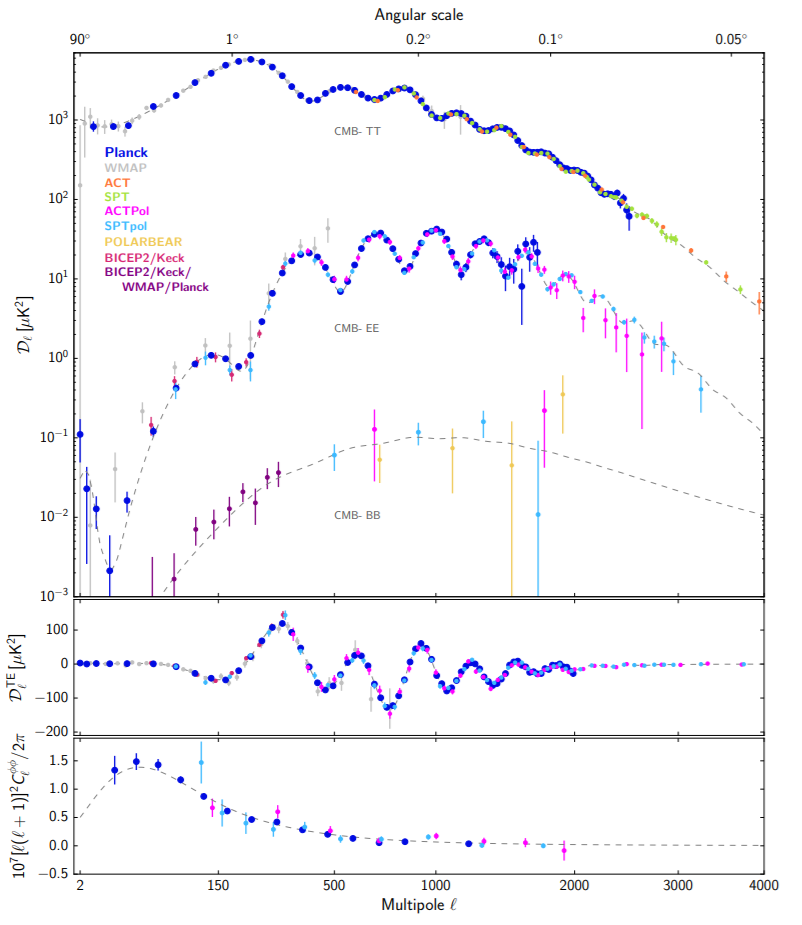
\includegraphics[width=0.85\textwidth]{cosmo_evol/CMB_compilation.png}
    \caption{Compilation of recent CMB angular power spectrum measurements from which most cosmological inferences are drawn.The upper panel shows the power spectra of the temperature and E-mode and B-mode polarization signals, the next panel the cross-correlation spectrum between T and E, while the lower panel shows the lensing deflection power spectrum. Different colours correspond to different experiments, each retaining its original binning. For Planck, ACTPol, and SPTpol, the EE points with large error bars are not plotted (to avoid clutter). The dashed line shows the best-fit \LCDM\ model to the Planck temperature, polarization, and lensing data. \textit{Note:} Reprinted from \textcite{2018arXiv180706205P}.}
    \label{fig:cmb_compilation}
\end{figure}
%%%%%%%%%%%%%%%%%%%%%%%
% Supernovae
%%%%%%%%%%%%%%%%%%%%%%%
\subsection{Supernovae}
Supernovae (SNe) are the most straightforward tool for studying cosmic acceleration, as they directly discovered the acceleration in the first place \parencite{riess}. Type Ia supernovae (SNe Ia) are exploding stars defined by the lack of hydrogen and the presence of silicon in their early-time spectra \parencite{SN}, and are a product of a thermonuclear explosion of a C/O white dwarf. Observations show that SNe Ia have a luminosity peak that is tightly correlated with the shape of their light curves -- supernovae that rise and fall more slowly have higher peak luminosity \parencite[first quantified by][]{SN_lum}. From observations of (multiband) light curve shapes and colors the luminosity at a brightness peak can be predicted.

To measure cosmic expansion with Type Ia SNe, the observed flux and predicted luminosity are compared. From that the supernova's luminosity distance can be measured. An accurate redshift is obtained by measuring the host galaxy (calibrator). Since the distances to the local calibrators are usually determined from the Hubble expansion, this method gives the luminosity distance $D_L$ in units of $h\mins$ Mpc. Measured relation is used to constraint dark energy parameters.

Recent analysis of \textcite{Abbott_2019} uses data from the Dark Energy Survey Supernova Program (DES-SN) -- 207 spectroscopically confirmed SNe Ia from the first three years of DES-SN combined with a low-redshift sample of 122 SNe from the literature. For a flat $w$CDM\ model they found a matter density $\Omega_m=0.321\pm0.018$ and an equation of state $w=-0.978\pm0.059$, see \autoref{fig:des_sne_results}.

\begin{figure}[hbt]
    \centering
    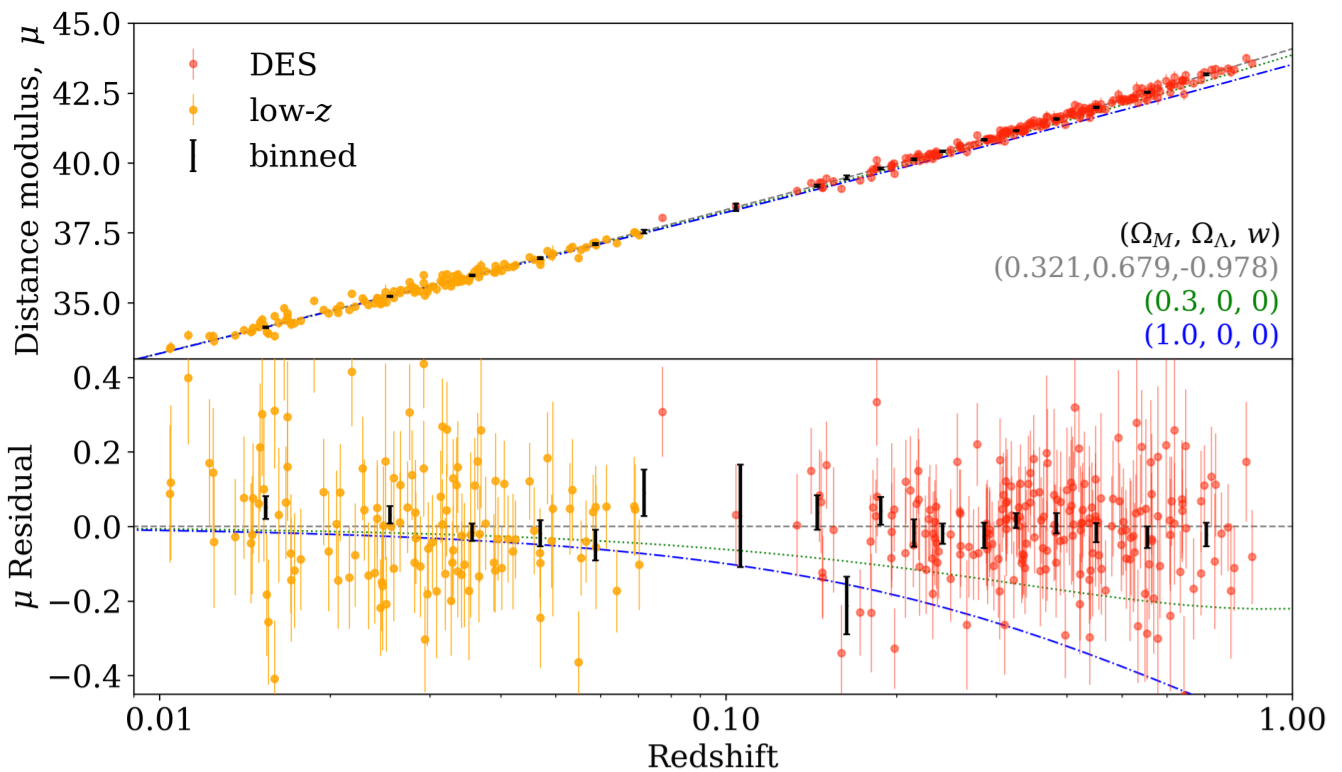
\includegraphics[width=0.7\textwidth]{cosmo_evol/DES_SNe_results.png}
    \caption{Hubble diagram for the DES-SN3YR sample. Top: distance modulus $(\mu =5\log [d_L/10\rm{pc}])$ from ``BEAMS with Bias Corrections'' fit \parencite{Kessler_2017}, black bars, which are used for cosmology fits) and for each SN (red, orange circles). The dashed gray line shows best fit model, while the green and blue dotted lines show models with no dark energy and matter densities $\Omega_m = 0.3$ and $1.0$ respectively. Bottom: residuals to the best fit model; $1\sigma$ error bars show 68\% confidence. \textit{Note:} Reprinted from \textcite{Abbott_2019}.}
    \label{fig:des_sne_results}
\end{figure}
%%%%%%%%%%%%%%%%%%%%%%%
% BAO
%%%%%%%%%%%%%%%%%%%%%%%
\subsection{Baryonic acoustic oscillations}
\label{sec:bao}
Baryonic acoustic oscillations (BAO) provide an entirely independent way of measuring cosmic distance. Sound waves propagating before recombination imprint a characteristic scale on matter clustering. The acoustic length scale can be computed as
\eq{
r_s=\int_0^{t_\ast}{\frac{c_s(t)}{a(t)}\dd t}=\int_{z_\ast}^{\infty}{\frac{c_s(z)}{H(z)}\dd z},
}
where asterisk denotes time (redshift) at recombination and $c_s$ is the sound speed. The behavior of $H(z)$ depends on the ratio of the matter density to radiation density and the sound speed depends on the ratio of radiation pressure to the energy density of the baryon-photon fluid, determined by the baryon-to-photon ratio. Both the matter-to-radiation ratio and the baryon-to-photon ratio can be measured from the CMB anisotropy power spectrum. This gives $r_s\sim150$ Mpc. The scale of the acoustic feature is stable to better than 1\% accuracy, making it an excellent standard ruler.

This effect can be detected in the angular clustering of galaxies in bins of photometric redshift, yielding the angular diameter distance. Furthermore, measuring the BAO scale in a velocity separation allows a direct determination of $H(z)$. The BAO method measures $D(z)$ in absolute units -- Mpc not $h\mins$ Mpc like SNe measurements, and thus BAO measurements to the same redshift carry different information. At low redshift $(z\lesssim0.5)$, the BAO method strongly complements SN measurements, while at higher redshift $(z\gtrsim0.5)$ the BAO method is an powerful probe of dark energy and cosmic geometry.

BAO can be clearly seen in the correlation function \parencite[see e.g.][]{1993ApJ...412...64L} for definition and estimators). The two-point correlation function $\xi(r)$ is the excess probability $\dd P$ of finding two pairs of galaxies in two volumes $\dd V_1$ and $\dd V_2$ at a given comoving distance $r$
\eq{
    \label{eq:corr}
    \dd P = \bar{n}^2[1+\xi(r)]\dd V_1 \dd V_2\,,
}
where $\bar{n}$ is the expected density of the distribution. The distances are usually measured using the redshift in the redshift space where the distortions (see \autoref{sec:rsd}) cause the redshift-space correlation $\xi(s)$ function to vary according to the angle between the separation vector and the line of sight. In \autoref{fig:xi_s} we see the spherically averaged correlation function from \textcite{2005ApJ...633..560E} with the clear bump at $100h^{-1}$ Mpc scale.
\begin{figure}[hbt]
    \centering
    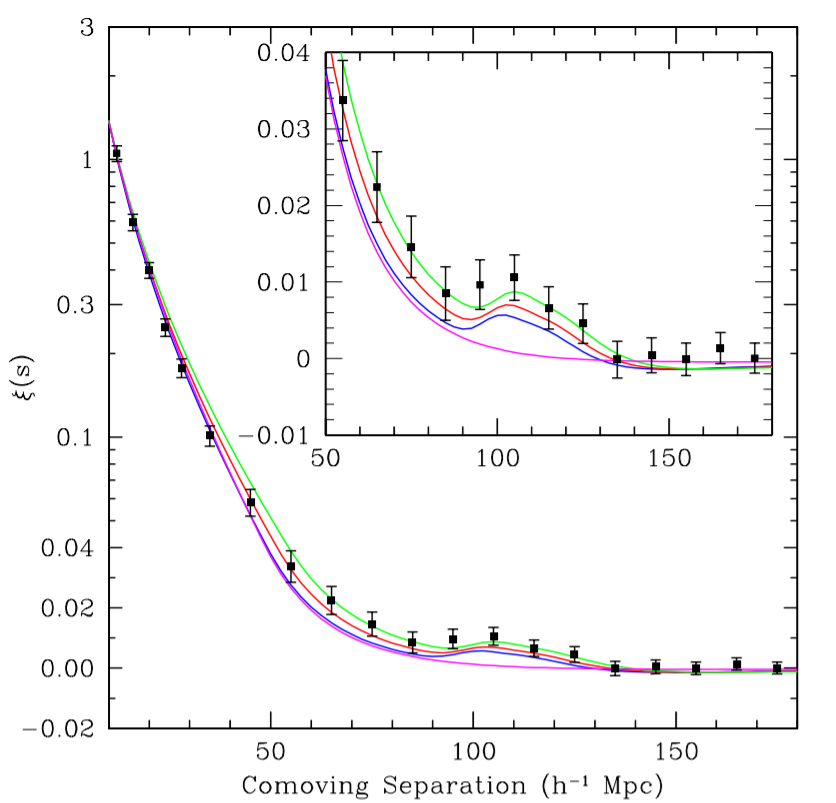
\includegraphics[width=0.7\textwidth]{cosmo_evol/bao_rsd.png}
    \caption{The large-scale redshift-space correlation function of the SDSS LRG sample. The error bars are from the diagonal elements of the mock-catalog covariance matrix; however, the points are correlated. Note that the vertical axis mixes logarithmic and linear scalings. The inset shows an expanded view with a linear vertical axis. The models are $\Omega_mh^2=0.12$ (top, green), $0.13$ (red), and $0.14$ (bottom with peak, blue), all with $\Omega_bh^2=0.024$ and $n=0.89$ and with a mild non-linear prescription folded in. The magenta line shows a pure CDM model ($\Omega_mh^2=0.105$), which lacks the acoustic peak. It is interesting to note that although the data appears higher than the models, the covariance between the points is soft as regards overall shifts in $\xi(s)$. Subtracting $0.002$ from $\xi(s)$ at all scales makes the plot look cosmetically perfect, but changes the best-fit $\chi^2$ by only $1.3$. The bump at$100h^{-1}$ Mpc scale, on the other hand, is statistically significant. \textit{Note:} Reprinted from \textcite{2005ApJ...633..560E}.}
    \label{fig:xi_s}
\end{figure}

In \textcite{BAO_results} present a measurement of the BAO from the three-dimensional correlation of Lyman-$\alpha$ forest absorption and quasars from the SDSS Data Release 14 (the first two years of observations by the eBOSS) at redshift $z=2.35$. The position of the BAO peak is used to determine the Hubble distance $d_H$ and the comoving angular diameter distance $d_A$ relative to the sound horizon at the drag epoch $r_s: d_H(z=2.35)/r_s = 9.20\pm0.36$ and $d_M(z=2.35)/r_s = 36.3\pm1.8$. These results are $1.5\sigma$ from the flat \LCDM\ model of \textcite{2016A&A...594A..13P}.
%%%%%%%%%%%%%%%%%%%%%%%
% WL
%%%%%%%%%%%%%%%%%%%%%%%
\subsection{Weak lensing}
Gravitational lensing is the deflection of light from distant sources due to the bending of space-time by baryonic and dark matter (lenses) along the line of sight. It is a very useful cosmological probe because it is sensitive to all matter regardless of its nature. In the limit of very small deflection angles it is called weak lensing (WL). WL causes tiny distortions ($\sim0.5\%$), or ``shear'', in galaxy sizes and shapes -- see \autoref{fig_WL_Abell}. Intrinsic size or shape of a given galaxy are unknown, but normally, galaxy orientations are assumed to be random ($\sim30\%$ dispersion), so they should not exhibit statistically significant and coherent alignments. In the presence of lensing, small but coherent shears in background galaxy images are induced. This means that WL is statistically detectable by averaging shapes over many lensed galaxies. In principle either the shearing of galaxies (shape distortion) or their magnification (size distortion) can be measured. However, in practice the shape distortions is used much more widely, since the scatter in shapes of galaxies is less than the scatter in their sizes.

Weak lensing provides a direct measure of the distribution of matter, independent of any assumptions about galaxy biasing. Since this distribution can be predicted theoretically, and its amplitude can be directly used to constrain cosmology, weak lensing has great potential as a cosmological probe. The correlation of the density field of nearby galaxies with the lensing shear measured on more distant galaxies is called \textit{galaxy-galaxy lensing}. Most lens systems involve sources (and lenses) at moderate or high redshift, and thus can lensing probe the geometry of the Universe -- the measurement of the shear correlation function as a function of the redshifts of observed galaxies is called \textit{tomography}. The scaling of the galaxy-galaxy lensing signal as a function of the source redshift, known as \textit{cosmography}, depends purely on geometric factors and hence can be used to construct a distance-redshift relation.
\begin{figure}
	\centering
		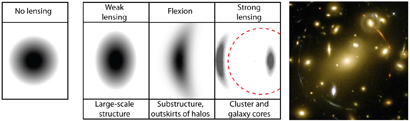
\includegraphics[scale=1.00]{cosmo_evol/WL_abel.jpg}
	\caption{(Left) Illustrations of the effect of a lensing mass on a circularly symmetric image. Weak lensing elliptically distorts the image, flexion provides an arc-ness and strong lensing creates large arcs and multiple images. (Right) Galaxy cluster Abell 2218, strongly lensed arcs can be seen in around the cluster. Every background galaxy is weakly lensed. \textit{Note:} From NASA, ESA, and Johan Richard (Caltech, USA).}
	\label{fig_WL_Abell}
\end{figure}
%%%%%%%%%%%%%%%%%%%%%%%
% Large-scale structure
%%%%%%%%%%%%%%%%%%%%%%%
\subsection{Large-scale structure}
Studying the large-scale structures (LSS) of the Universe is of a great importance for the cosmology. Since the clustering of matter on scales from galaxies to superclusters came from quantum fluctuations in the very early Universe with important modification by radiation and baryons, the LSS encode critical information about the contents of the Universe, the origin of the fluctuations, and the cosmic expansion background in which the structures evolved.

Measurements of large-scale power spectrum for the spatial distribution of matter as a function of redshift constrain the cosmic expansion history, the cosmological distance scale, the growth rate of structures, the mass of the neutrinos and the abundance of dark matter. This includes BAO measurement of the distance-redshift relation (as a standard ruler). The BAO with the growth of the LSS in the Universe form two robust probes of dark energy, and a potential discriminator between dark energy and modified gravity models. Beyond the dark energy, the large scale power spectrum is a probe of both neutrino mass and primordial non-gaussianity.
\subsubsection{Matter power spectrum}
The matter power spectrum $P(k)$ is defined as a quadratic function of the Fourier transformation of the density contrast $\delta$
\eq{
  \label{eq:pk}
  P(k)(2\pi)^3\delta_{\rm D}(k-k')\equiv \left\langle \hat\delta(k)\hat\delta^*(k')\right\rangle\,,
}
where $\delta_{\rm D}$ is the Dirac delta function and we are averaging over possible realizations. The power spectrum is by far the most common descriptor of clustering in the linear and mildly non-linear regime and plays a central role in cosmology. The power spectrum is the Fourier transform of the correlation function \eqref{eq:corr}
\eq{
    \label{eq:pk_xi}
    P(k)=\int\xi(r)e^{-ik\cdot r}\dd^3r\,.
}
However what we observe in practice is the galaxy density contrast $\delta_g$, which is different from the total matter density contrast $\delta_m$. The two quantities are assumed to be related by a bias factor $b$ defined by
\eq{
    b\equiv\frac{\delta_g}{\delta_m}\,,
}
from which follows $P_g(k)=b^2P_m(k)$. The idea of a simple biasing scheme tries to capture physics beyond the purely linear gravitational treatment, e.g. merging processes or evolutionary processes that render galaxies brighter or dimmer and therefore visible or invisible to our telescopes.

In \autoref{fig:pk_planck} is shown (linear) matter power spectrum inferred from different cosmological probes \parencite{2018arXiv180706205P}.
\begin{figure}[hbt]
    \centering
    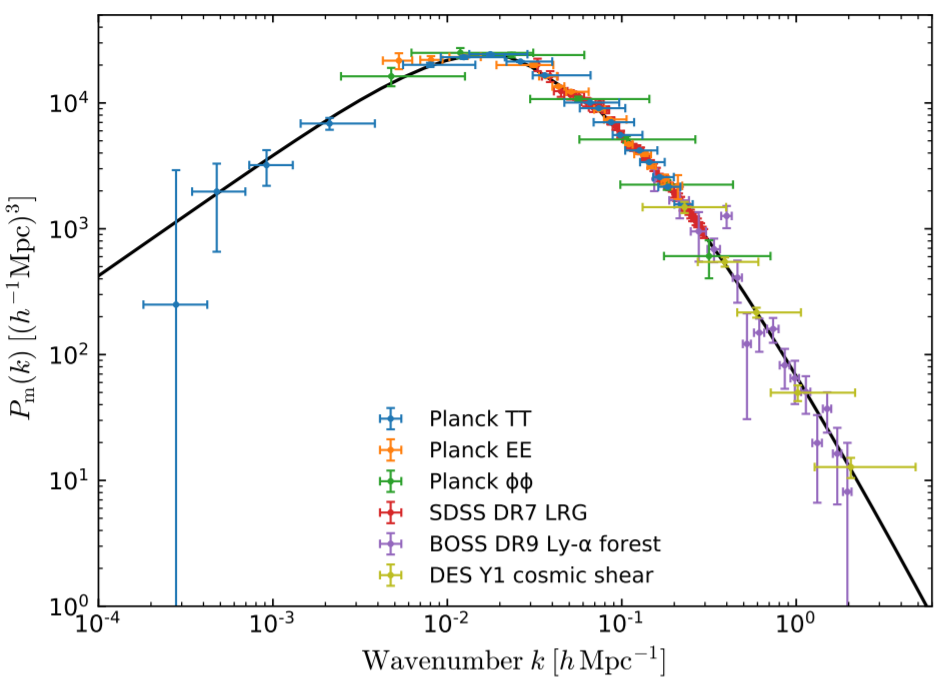
\includegraphics[width=0.7\textwidth]{cosmo_evol/pk_planck.png}
    \caption{The (linear theory) matter power spectrum (at z = 0) inferred from different cosmological probes. The broad agreement of the model (black line) with such a disparate compilation of data, spanning 14 Gyr in time and three decades in scale is an impressive testament to the explanatory power of \LCDM. Earlier versions of similar plots can be found in, for example, \textcite{1994ARA&A..32..319W}, \textcite{1995Sci...268..829S}, \textcite{2002PhRvD..66j3508T}, and \textcite{2004ApJ...606..702T}. A comparison with those papers shows that the evolution of the field in the last two decades has been dramatic, with \LCDM\ continuing to provide a good fit on these scales. \textit{Note:} Reprinted from \textcite{2018arXiv180706205P}.}
    \label{fig:pk_planck}
\end{figure}

%%%%%%%%%%%%%%%%%%%%%%%
% Galaxy clusters
%%%%%%%%%%%%%%%%%%%%%%%
\subsection{Galaxy clusters}
The observed number density and clustering of galaxy clusters as a function of mass and redshift provides a powerful toolset to constraining cosmology.  Galaxy clusters provided the first line of evidence for the existence of dark matter \textcite{zwicky} and cluster mass-to-light ratio measurements suggested that the matter density in the universe was sub-critical \textcite{Gott}. Galaxy clusters measurements are sensitive to both the expansion history and the growth of structure in the Universe enabling to distinguish between dark energy and modified gravity models for cosmic acceleration. Additional probes are measurements of the baryonic mass fraction in clusters, and of the tomographic lensing signatures through clusters.

The basic idea of cluster abundance studies is to compare the predicted space density of massive halos to the observed space density of clusters. The basic observables are the richness, the number of galaxies in a specified luminosity and color range. Halo abundance is sensitive to the amplitude of the matter power-spectrum $\sigma_8$ and the matter density $\Omega_m$, more precisely a combination of a form $\sigma_8\Omega_m^q$, with $q\approx0.4$ \textcite{white}. The degeneracy between $\sigma_8$ and $\Omega_m$ can be broken by measuring abundances at a variety of masses.
% \subsubsection{Spherical collapse}
% If we assume a spherical overdensity of pressureless matter in an expanding Universe we can arrive to the following equation \parencite{2010deto.book.....A}
% \eq{
%     \delta''+\left(1+\frac{\HH'}{\HH}\right)\delta'-\frac32\Omega_m\delta=\frac43\frac{\delta'^2}{1+\delta}+\frac32\Omega_m\delta^2\,,
% }
% which has a solution in the Einstein--de Sitter Universe
\subsubsection{The halo mass function}
The halo mass function (HMF) $\dd n/\dd M$ is defined as the number of haloes of mass $M$ per unit volume per unit interval in $M$. To describe the halo mass function we need two other quantities, $f(\sigma)$ and $\ln\sigma^{-1}$. The rms linear overdensity $\sigma$ of the density field smoothed with a top-hat filter $W$ with a radius that encloses a mass $M$ at the mean cosmic matter density is defined as
\eq{
    \sigma^2(M, z)=\frac{D^2(z)}{2\pi^2}\int_0^\infty{k^2P(k)W^2(k,M)\dd k}\,.
}
The mass function is then written as
\eq{
    \label{eq:hmf}
    \dddd nM=\frac{\rho_0}{M}\dddd{\ln\sigma^{-1}}{M}f(\sigma)\,,
}
where all the cosmological information is contained in the function \(f(\sigma)\) --  the fraction of mass in collapsed haloes per unit interval in $\ln\sigma$. This function depends on how haloes are defined, usually using the friends-of-friends (FoF) algorithm of \textcite{1985ApJ...292..371D}. The analytical form of $f(\sigma)$ using the assumption of collisionless spherical collapse has been proposed by \textcite{1974ApJ...187..425P}
\eq{
    f_{PS}(\sigma) = \sqrt{\frac2\pi}\frac{\delta\coll}{\sigma}\exp{\left(-\frac{\delta\coll^2}{2\sigma^2}\right)}\,,
}
where the parameter \(\delta\coll=1.686\) introduced in the previous section can be interpreted physically as the linearly extrapolated overdensity of a top-hat spherical density perturbation at the moment of maximum compression for an Einstein de-Sitter universe. While as a first approximation the PS mass function agrees with simulations at $z=0$ reasonably well, it overpredicts the number of low-mass halos and underpredicts the number of massive halos at the current epoch. \textcite{2001MNRAS.321..372J} combined high-resolution simulations for four different CDM cosmologies spanning a mass range of over 3 orders of magnitude $(\sim10^{12}-10^{15}h^{-1}M_\odot)$, and including several redshifts $z=0-5$. They came up with the following fitting function
\eq{
    \label{eq:hmf_jenkins}
    f_{Jenkins}(\sigma)=0.315\exp\left(-|\ln\sigma^{-1}+0.61|^{3.8}\right)\,.
}
As their range of masses and redshifts correspond to our study case we will use this fitting formula in our analysis (see \autoref{chpt:app_sims}).
%%%%%%%%%%%%%%%%%%%%%%%
% Strong lensing
%%%%%%%%%%%%%%%%%%%%%%%
\subsection{Strong lensing}
Strong gravitational lensing (SL) refers to the multiple imaging of a background object due to a massive foreground object (typically clusters of galaxies) -- see \autoref{fig_WL_Abell}. The resulting angular displacement, morphological distortion, and time delay can be used to measure dark energy parameters. Strong gravitational lensing time delays measure a combination of distances that combining with other dark energy probes can further constraint cosmological parameters. The time delays is also expected to test gravity on scales where the screening mechanisms is becoming active.

Another independent way to measure dark energy parameters with SL is the analysis of systems with multiple sets of multiple images \textcite{SL_in_CLGs}. The positions of these multiple images depend strongly on the detailed properties of the lens mass distribution and on the angular diameter distance ratios between the lens, source and observer, they encapsulate information about the underlying cosmology. This dependence on the geometry can be used to derive constraints on the cosmological parameters.
%%%%%%%%%%%%%%%%%%%%%%%
% Redshift-space distortions
%%%%%%%%%%%%%%%%%%%%%%%
\subsection{Redshift-space distortions}
\label{sec:rsd}
When we observe distant galaxies, two features determine their redshifts -- the Hubble expansion and their peculiar velocities. The peculiar velocities of galaxies thus cause them to appear displaced along the line of sight in redshift space. These displacements lead to redshift distortions in the pattern of clustering of galaxies in redshift space and make large scale galaxy clustering anisotropic. Redshift-space distortions (RSD) have the tremendous advantage of bearing information about the dynamics of galaxies.

The coordinate transformation from real space $(r)$ to redshift space $(s)$ of a source with a peculiar velocity $\bm v$ is given by
\eq{
    \mb s = \mb r\left[1+\frac{u(r)-u(0)}{r}\right]\,,
}
whre $u\equiv\mb v\cdot\mb r/r$. The strength of the anisotropy is governed by distortion parameter $\beta = f(z)/b(z)$, where $f(z)$ is the logarithmic growth rate of fluctuations \eqref{eq:grw_rate} and $b$ is the bias. By modeling the full redshift-space galaxy power spectrum one can obtain combination of the product of the matter clustering amplitude and the growth rate.

Anisotropy of galaxy clustering offers an alternative to weak lensing and cluster abundances as a tool for measuring the growth of structures. RSD directly measure the rate at which structure is growing at the redshift of observation unlike WL and galaxy cluster measurements  which measure the rate of growth at multiple redshifts. RSD measurements can improve constraints on dark energy models and they can be used to constrain departures from GR by testing consistency of the growth and expansion histories. The key challenge in modeling RSD is accounting for non-linear effects, including non-linear or scale-dependent bias between galaxies and matter, at the level of accuracy demanded by the LSST`s precision.